\chapter{Results}

I analysed three daily networks, these are refererred to below as \#1, \#2, and \#3. Each network is aggregated for ten hours starting at 8~a.m. and lasting until 6~p.m. I chose the 20.08.2016, 22.08.2016, and 24.08.2016, because at this point in time the hive also contained tagged foragers (older bees). At the same time young bees were added to the colony (see table~\ref{tab:networks} for details). The age distribution for each network is shown in figure~\ref{fig:ages}.

[TODO: PLOT How many nodes in the network stay the same over 3 timesteps? (will be going next step, same, new ones)]

\begin{table}
\centering
\begin{tabular}{ccccccc}
\toprule
{} & 20.08.16 & 21.08.16 & 22.08.16 & 23.08.16 & 24.08.16 \\
\midrule
Network ID & \#1 & - & \#2 & - & \#3 & \\
Number of added bees & 0 & 0 & 110 & 60 & 0 \\
Time added & - & - & 2~p.m. & 6~p.m. & - \\
\bottomrule
\end{tabular}
\caption[TODO]{Overview about networks and number of added bees.}
\label{tab:networks}
\end{table}

\begin{figure}[htb]
	\centering
	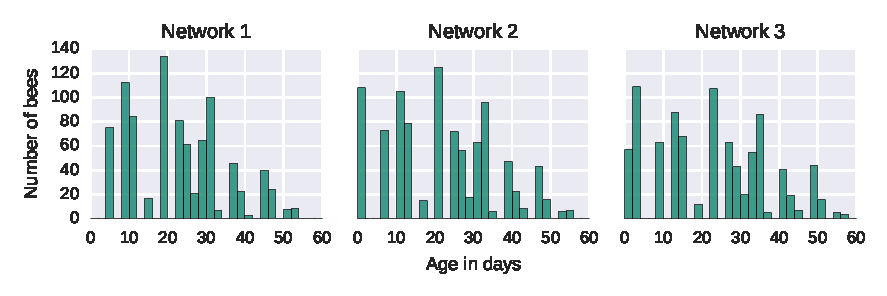
\includegraphics[width=1.0\textwidth]{Figures/ages}
	\caption[Age distribution per network]{Age distribution per network: The width of a bar corresponds to two days.}
	\label{fig:ages}
\end{figure}

\section{Network type and properties}
 
\subsection{Global Structure - Network Level}
Each network consists of one giant component. Table~\ref{tab:stats} summarizes basic network properties number of nodes, number of links, density, diameter, average shortest path length, global clustering coefficient, average degree, and average strength.\\

TODO: high density, small diameter, very short average path length, high clustering coefficient, high strength and degree, compared to what? random graph\\

TODO: calc network centralisation and add to table\\
TODO: PLOT degree and strength distribution\\
TODO: PLOT edge weight distribution\\

\begin{table}
\centering
\begin{tabular}{lcccccccc}
\toprule
{} &  $N$ &   $L$ &  $D$ &  $\langle d_{\texttt{max}} \rangle$ &  $\langle d \rangle$ &   $C_\Delta$ &  $\langle k \rangle$ &  $\langle s \rangle$ \\
\midrule
\#1 &    922 &  291179 &     0.69 &         3 &              1.32 &  0.79 &      631.62 &      5680.17 \\
\#2 &    978 &  256066 &     0.54 &         3 &              1.46 &  0.72 &      523.65 &      3977.94 \\
\#3 &    922 &  259421 &     0.61 &         3 &              1.39 &  0.75 &      562.74 &      4205.99 \\
\bottomrule
\end{tabular}
\caption[Global network properties]{Global network properties}
\label{tab:stats}
\end{table}

\subsection{Local Structure - Node Level}

[TODO: PLOT closeness, betweenness, local clustering coefficient, eigenvector centrality, weighted and unweighted]

\subsection{Network type}

[TODO: compare to random graph]\\
degree distribution random poisson or binominal, not random power law\\
giant component, connectedness\\
average path length and diameter very small, small world phenomenon\\
higher clustering coefficient than in random\\

\section{Network Metrics in Relation to Age of Bees}

[TODO: all plot in relation to age]

\section{Community Detection}

TODO: if time: show that communities are robust in terms of ilen.\\
TODO: age: müsste man eigentlich nochmal gegen ein randomisiertes Modell testen. Alter randomisieren\\
TODO: Communities centrality testen\\

Using the leading eigenvector (LE) algorithm in all three networks two communities with about the same number of nodes are detected. With walktrap in network 1 two communities and in network 2 and 3, three communities. The exact number of community members for algorithm is shown in table~\ref{tab:networks}.

The first community (LE-C1, WT-C1) contains the queen and bees who are on average younger than the second community (LE-C2, WT-C3). For walktraps third community it is a middle-aged community (WT-C2). The age difference for network 1 is $8.4$ days, for network 2 $10.9$ days, and for network 3 $14.4$ days on average for leading eigenvector communities.

The age distribution for each community and network is depicted in figure~\ref{fig:ageDistribution}.

A two sample Kolmogorov–Smirnov test showed, that for leading eigenvector communities, the age distributions are significantly different ($p< 0.001$). For walktrap C1 with C2 and C3 are significantly different, but C2 and C3 are not that much significant. Exact $p$-values are shown in table~\ref{tab:pvalues2}

\begin{table}
\centering
\caption[Overview about communities]{\textbf{Overview about communities per network} Communities marked with * contain the queen. Age and standard deviation (SD) are measured in days.}
\label{tab:communities}
\vspace*{5mm}
\begin{tabular}{lcrrrrr}
	\toprule
	{}  & ID & Members & Proportion & Age & SD\\
	\midrule
	\rowcolor{Gray}
	Leading eigenvector &&&&&\\
	\midrule 
	\quad Network 1  & C1 & $*434$  & 47.07\% & $16.81$ & $\pm17.91$ \\
	                 & C2 & $488$   & 52.93\% & $25.15$ & $\pm19.49$ \\
	\midrule   							
	\quad Network 2  & C1 & $*503$  & 51.43\% & $15.44$ & $\pm19.54$ \\
	                 & C2 & $475$   & 48.57\% & $26.37$ & $\pm18.01$ \\
	\midrule  
	\quad Network 3  & C1 & $*385$  & 41.76\% & $12.85$ & $\pm20.24$ \\
	                 & C2 & $537$   & 58.24\% & $27.26$ & $\pm17.84$ \\
    \midrule
    \rowcolor{Gray}
    Walktrap &&&&&\\
    \midrule 
	\quad Network 1 & C1 & $*431$ & 46.75\% & $16.76$ & $\pm17.92$\\
	                & C2 & $490$  & 53.15\% & $25.16$ & $\pm19.48$\\
	\midrule
	\quad Network 2 & C1 & $*372$ & 38.04\% & $12.98$ & $\pm19.00$\\
				    & C2 & $311$  & 31.80\% & $23.11$ & $\pm19.48$\\
				    & C3 & $294$  & 30.06\% & $28.15$ & $\pm16.77$\\            
	\midrule
	\quad Network 3 & C1 & $*231$  & 25.05\% & $7.09$  & $\pm19.60$\\
					& C2 & $301$  & 32.65\% & $23.83$ & $\pm17.22$\\
					& C3 & $390$  & 42.30\% & $27.63$ & $\pm18.48$\\
	\bottomrule
\end{tabular}
\end{table}

\begin{table}
\centering
\caption[Kolmogorov-Smirnov test]{\textbf{Kolmogorov-Smirnov test} $p$-values for leading eigenvector (LE) and walktrap (WT) for each network and its communities.}
\label{tab:pvalues2}
\vspace*{5mm}
\begin{tabular}{lcrrrrr}
	\toprule

	\rowcolor{Gray}
	 & & LE p-value & WT p-value\\
	\midrule 
	\quad Network 1  & C1, C2 & 5.1e-32 & 3.3e-31 \\
	\midrule   							
	\quad Network 2  & C1, C2 & 7.6e-38 & 2.3e-32 \\
					    & C1, C3 & & 1.3e-44\\
					    & C2, C3 & & 6.6e-05\\
	\midrule  
	\quad Network 3  & C1, C2 & 1.4e-64 & 1.8e-65\\
					    & C1, C3 & &3.9e-93\\
						& C2, C3 & &2.6e-05\\ 
	\bottomrule
\end{tabular}
\end{table}


\begin{figure}[htb]
	\centering
	\begin{subfigure}[b]{1.0\textwidth}
		\centering
		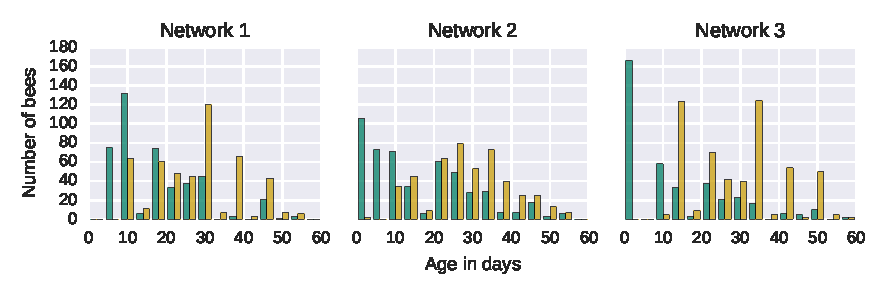
\includegraphics[width=1.0\textwidth]{Figures/ageDistribution-LE}
		\caption[Leading eigenvector]{Leading eigenvector}
		\label{fig:ageLE}
		\vspace*{5mm}
	\end{subfigure}
	%\vspace{1cm} 
	\begin{subfigure}[b]{1.0\textwidth}	
		\centering
		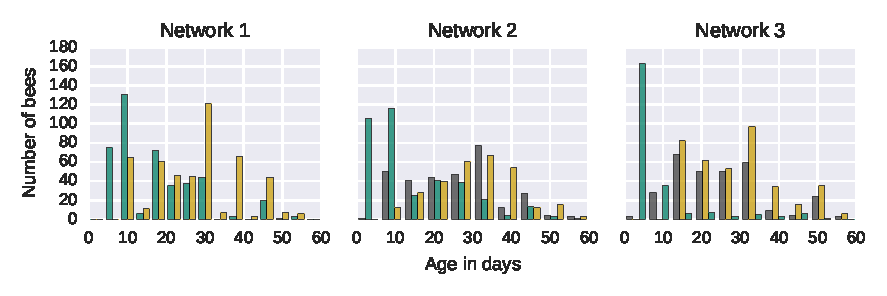
\includegraphics[width=1.0\textwidth]{Figures/ageDistribution-WT}
		\caption[Walktrap]{Walktrap}
		\label{fig:ageWT}
		\vspace*{5mm}
	\end{subfigure}
	%\vspace{1cm}
	\caption[Age distribution for each community and network] {\textbf{Age distribution for each community and network} The \emph{green} bar is the community containing the queen. The queens age is not included in the statistic. The \emph{orange} bars coresspond to the second community, containing older bees. The \emph{gray} bars is a third community only revealed by walktrap and contains middle-aged bees.}
	\label{fig:ageDistribution}
\end{figure}


\subsection{Spatial Distribution of Communities}
The two communities detected by leading eigenvector are located in two different regions of the honeycomb. The older community (\emph{orange} in figure~\ref{fig:communitiesPerNetworkLE})) is in all three networks closer to the hive exit and the younger community (\emph{green} in figure~\ref{fig:communitiesPerNetworkLE})) is situated in the comb center.
Walktrap revealed the same two communities like leading eigenvector for all three networks, with the same spatial distribution. For network 2 and 3, a third community (\emph{gray} in figure~\ref{fig:communitiesPerNetworkWT})) is located between the young and old community.

\begin{figure}[htb]
	\centering
	\begin{subfigure}[b]{1.0\textwidth}
		\centering
		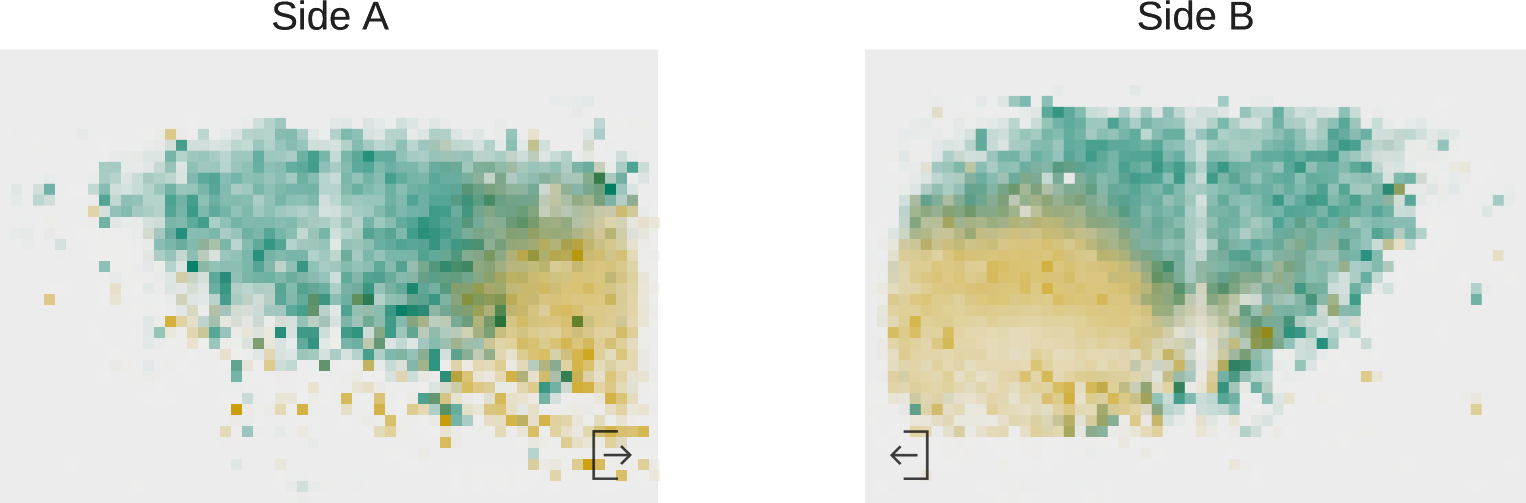
\includegraphics[width=\textwidth]{Figures/le_network1}
		\caption[Network 1]{Network 1}
		\label{fig:le1}
		\vspace*{5mm}
	\end{subfigure}
	%\vspace{1cm} 
	\begin{subfigure}[b]{1.0\textwidth}
		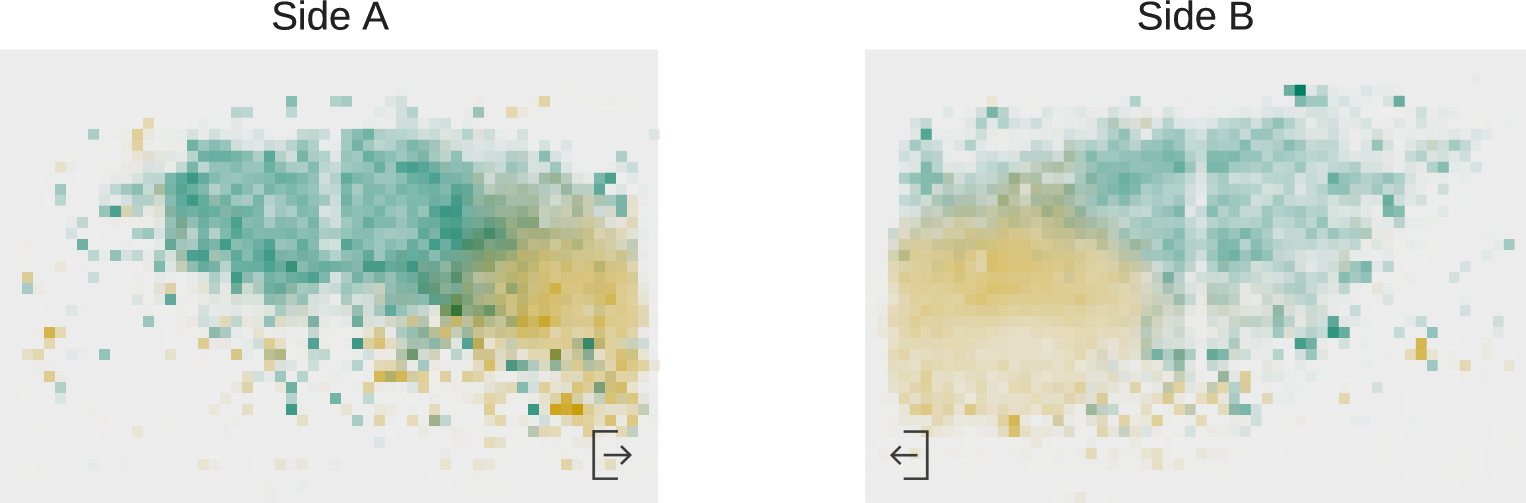
\includegraphics[width=\textwidth]{Figures/le_network2}
		\caption[Network 2]{Network 2}
		\label{fig:le2}
		\vspace*{5mm}
	\end{subfigure}
	%\vspace{1cm} 
	\begin{subfigure}[b]{1.0\textwidth}
		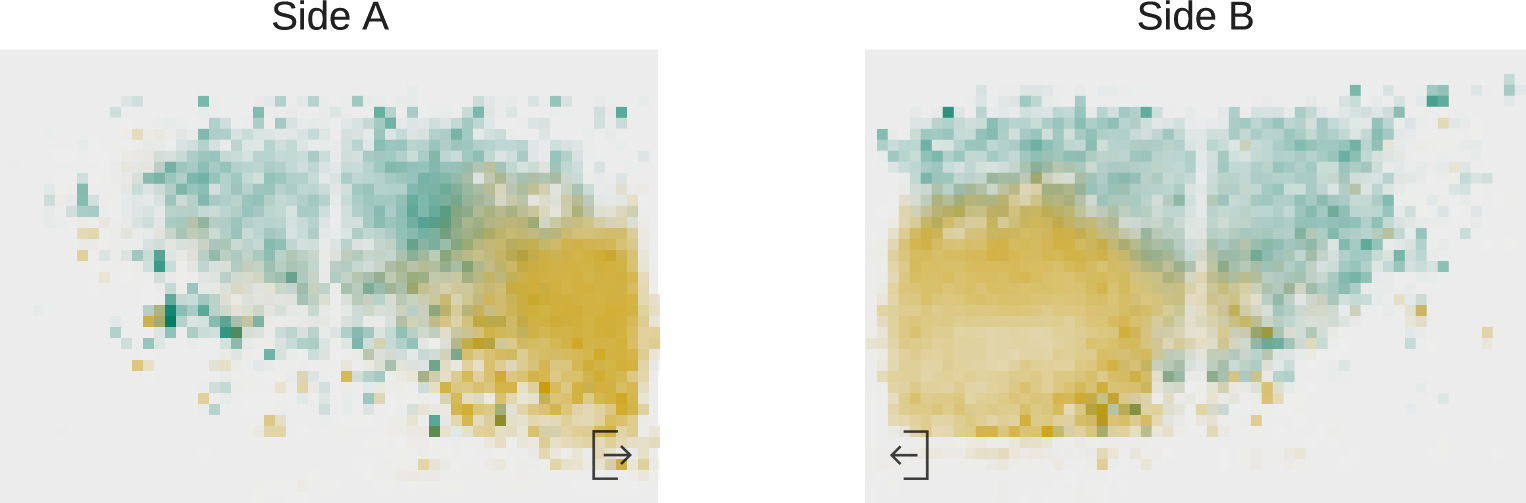
\includegraphics[width=\textwidth]{Figures/le_network3}
		\caption[Network 3]{Network 3}
		\label{fig:le3}
		\vspace*{5mm}
	\end{subfigure}
	\caption[Communities per network - leading eigenvector]{\textbf{Communities per network - leading eigenvector} The \emph{green} colour represents the younger community, containing the queen. The \emph{orange} color represents the older community. The hive exit on side A is on the bottom right and on side B on the bottom left. The data is aggredated for the complete timeframe of ten hours.}
	\label{fig:communitiesPerNetworkLE}
\end{figure}

\begin{figure}[htb]
	\centering
	\begin{subfigure}[b]{1.0\textwidth}
		\centering
		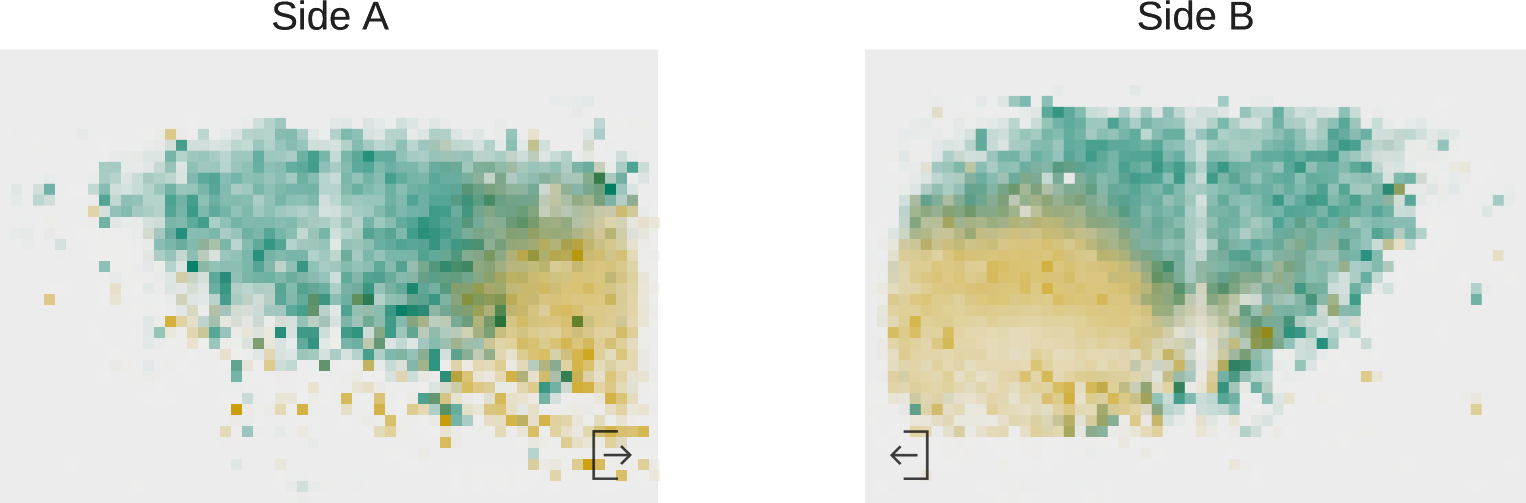
\includegraphics[width=\textwidth]{Figures/wt_network1}
		\caption[Network 1]{Network 1}
		\label{fig:wt1}
		\vspace*{5mm}
	\end{subfigure}
	%\vspace{1cm} 
	\begin{subfigure}[b]{1.0\textwidth}
		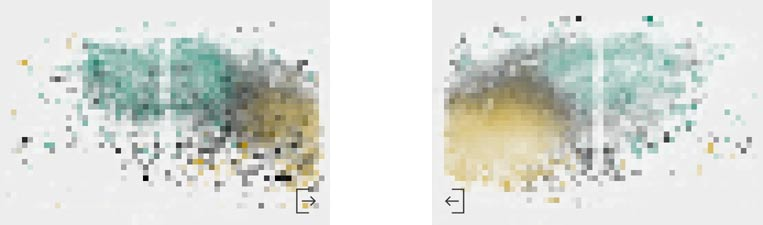
\includegraphics[width=\textwidth]{Figures/wt_network2}
		\caption[Network 2]{Network 2}
		\label{fig:wt2}
		\vspace*{5mm}
	\end{subfigure}
	%\vspace{1cm} 
	\begin{subfigure}[b]{1.0\textwidth}
		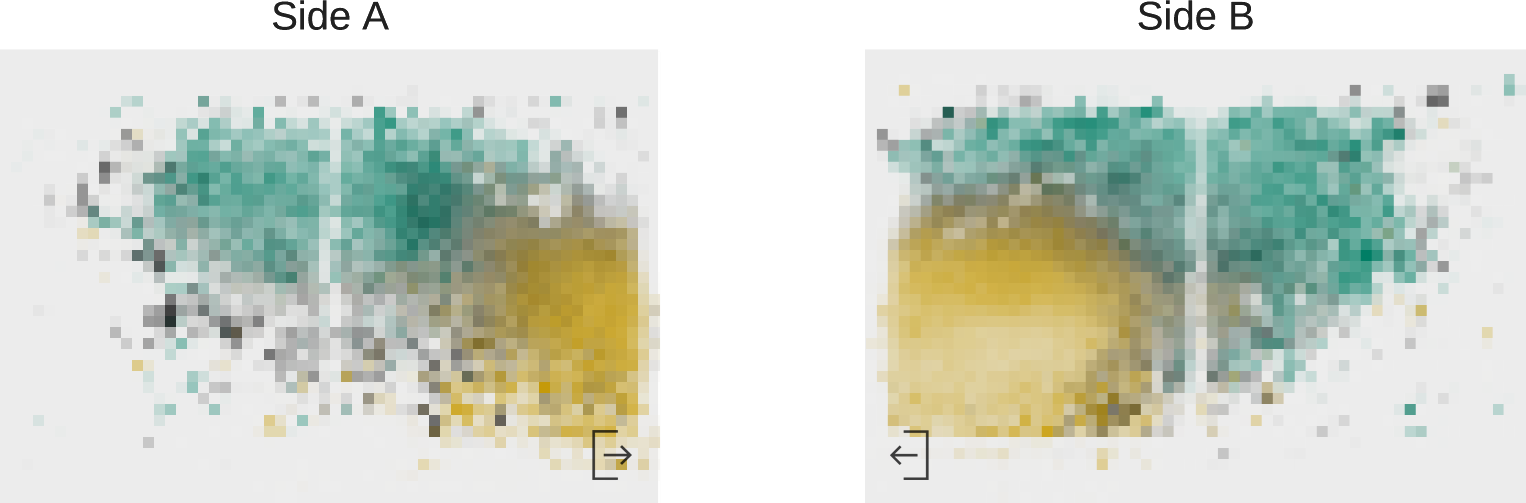
\includegraphics[width=\textwidth]{Figures/wt_network3}
		\caption[Network 3]{Network 3}
		\label{fig:wt3}
		\vspace*{5mm}
	\end{subfigure}
	\caption[Communities per network - walktrap]{\textbf{Communities per network - walktrap} The \emph{green} colour represents the younger community, containing the queen. The \emph{orange} color represents the older community. The \emph{gray} represents the middle-age community. The hive exit on side A is on the bottom right and on side B on the bottom left. The data is aggredated for the complete timeframe of ten hours.}
	\label{fig:communitiesPerNetworkWT}
\end{figure}


\subsection{Community members over time}
The match value between the two communities in successive time steps are calculated with formula~(\ref{eq:match}) and presented in figure~\ref{fig:membersLE} for the resulting communities using the leading eigenvector algorithm and figure~\ref{fig:membersWT} for the communities detected with walktrap.

\begin{figure}[htb]
	\centering
	\begin{subfigure}[b]{1.0\textwidth}
	\centering
	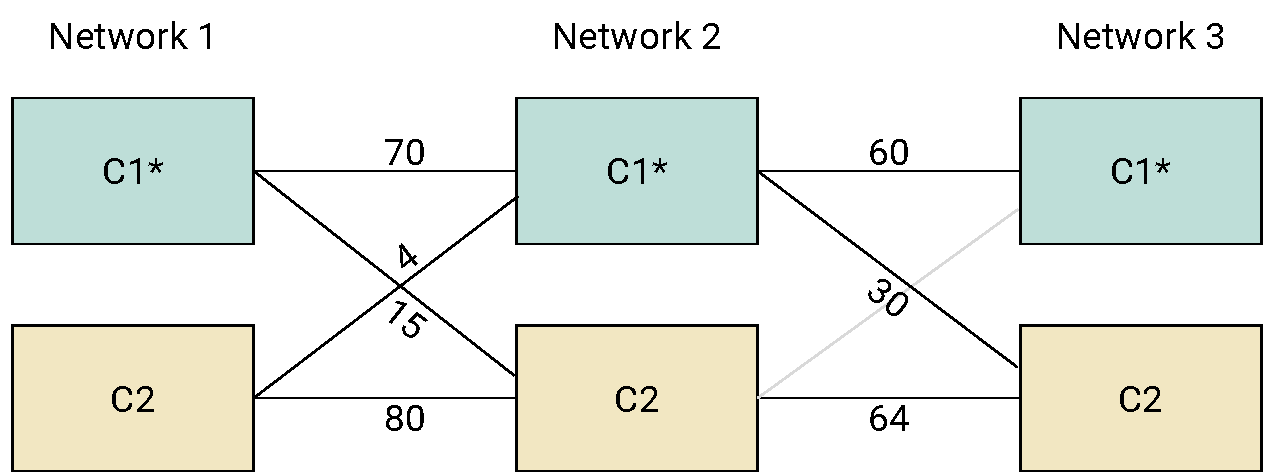
\includegraphics[width=.8\textwidth]{Figures/membersLE}
	\caption[Leading eigenvector communities]{Leading eigenvector communities}
	\label{fig:membersLE}
	\vspace*{5mm}
	\end{subfigure} 
	\begin{subfigure}[b]{1.0\textwidth}
	\centering
	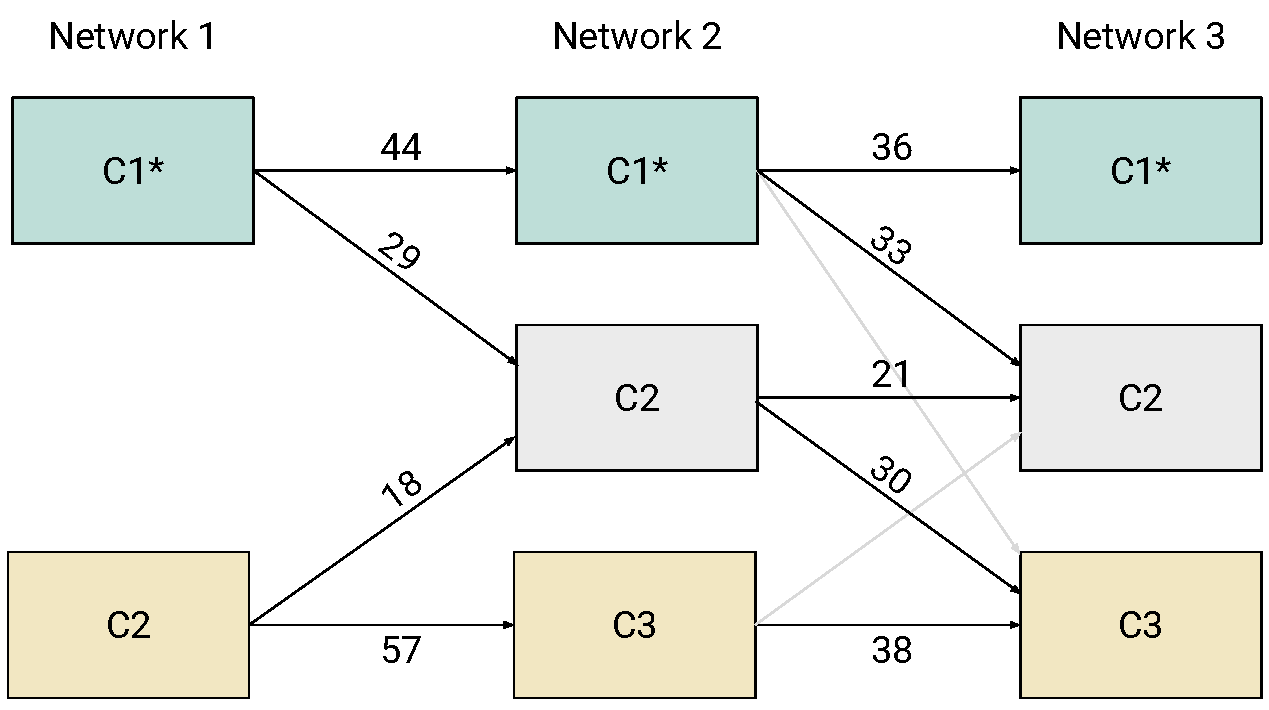
\includegraphics[width=.8\textwidth]{Figures/membersWT}
	\caption[Walktrap communities]{Walktrap communities}
	\label{fig:membersWT}
	\vspace*{5mm}
	\end{subfigure}
	\caption[Community matching]{\textbf{Community matching} The numbers indicate the match values in percent. The community marked with * contains the queen. \emph{Green} represents the younger community \emph{orange} the older community, and gray the middle-aged community. The light gray arrow represents match values below three percent.}
	\label{fig:members}
\end{figure}

\section{Summary}
TODO